% Provenance (never printed): lycee terminale S SVT "Les climats de la Terre"
% and the 2019 enseignement scientifique ("Le climat de la Terre": forcing,
% feedbacks, the IPCC assessments, scenarios), union; physical science only,
% as the user ruled (2026-10-22). See sources/outline_sources.md. Pilot
% chapter, 2026-10-22. Every figure about the climate system is an IPCC AR6
% WG1 statement (ledger ipcc:*) or computed from a dataset in
% figdata/grade-12/climate_records.py.
\chapter{Le changement climatique~: observations, causes et projections}\label{ch:g12:climate-change}

Haut sur le versant nord du Mauna Loa, un volcan situé au milieu de l'océan
Pacifique, un groupe de bâtiments blancs se dresse sur la lave nue, à
\qty{3397}{m} au-dessus de la mer. Là-haut, au-dessus de la couche d'air
polluée par l'île située en contrebas et à des milliers de kilomètres de
toute grande ville, l'air est à peu près aussi propre et aussi bien mélangé
que l'atmosphère de la planète entière. Depuis mars 1958, on y mesure son
dioxyde de carbone presque sans interruption. L'enregistrement a commencé
comme le projet d'un chimiste~; il est devenu la courbe la plus célèbre des
sciences de la Terre. Ce chapitre lit cette courbe et les autres
enregistrements du climat, explique comment un changement de l'air modifie
le \omterm{def:g10:earth-energy-budget:energy-budget}{bilan énergétique} de la planète, comment les scientifiques établissent
la cause du réchauffement qu'ils observent, et ce qu'ils projettent pour les
décennies à venir.
% ledger: noaa:mlo-site, noaa:keeling-1958

\begin{omfigure}
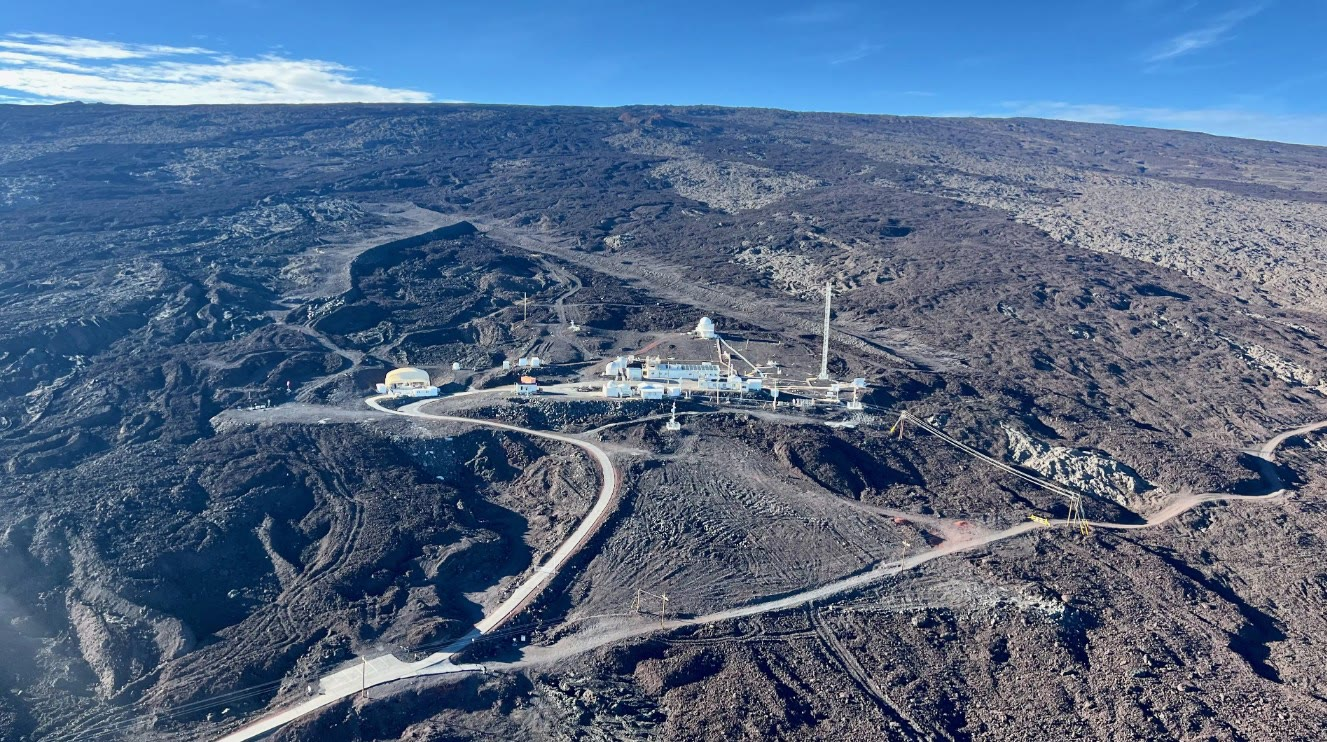
\includegraphics[width=0.78\linewidth]{images/book2/g12-noaa-mauna-loa-observatory.jpg}

{\small L'observatoire du Mauna Loa, à Hawaï, sur d'anciennes coulées de
lave, haut sur le flanc nord du volcan. Photographie~: Brian Vasel, NOAA
(domaine public).}
\end{omfigure}

\begin{recall}
La Terre reçoit de l'énergie du Soleil sous forme de lumière et en perd en
moyenne autant vers l'espace sous forme de rayonnement infrarouge~; la
fraction de la lumière solaire réfléchie est l'\omterm{def:g10:earth-energy-budget:albedo}{albédo}
(\cref{ch:g10:earth-energy-budget}). Les gaz à effet de serre --- vapeur
d'eau, dioxyde de carbone, méthane --- absorbent une partie de
l'infrarouge émis par la surface et en renvoient une partie vers le bas~;
cet effet de serre maintient la surface bien plus chaude qu'elle ne le
serait autrement (les livres de chimie, et le livre~1, année~9). Les
\omterm{def:g12:past-climates:ice-core}{carottes de glace} gardent des bulles d'air ancien et enregistrent les
\omterm{def:g12:past-climates:glacial-cycle}{cycles glaciaires} des 800\,000 dernières années
(\cref{ch:g12:past-climates}).
\end{recall}

\section{Les enregistrements}

\begin{omfigure}
\begin{tikzpicture}
\begin{axis}[omrecord, width=0.92\linewidth, height=6.2cm, xmin=1957, xmax=2028,
  ymin=305, ymax=440, xlabel={année}, ylabel={dioxyde de carbone (ppm)},
  xtick={1960,1970,...,2020}, /pgf/number format/1000 sep={}]
\addplot[omDef!85!black, line width=0.5pt] table[x=decimal_year, y=co2_ppm] {figdata/out/grade-12-climate_records-co2.dat};
\addplot[only marks, mark=*, mark size=0.9pt, omThm!85!black] table[x=year, y=co2_ppm] {figdata/out/grade-12-climate_records-co2annual.dat};
\end{axis}
\end{tikzpicture}

{\small La teneur de l'air en dioxyde de carbone au Mauna Loa~: moyennes
mensuelles (trait) et moyennes annuelles (points), en parties par million
(ppm) d'air sec. Données~: NOAA Global Monitoring Laboratory et Scripps
Institution of Oceanography.}
\end{omfigure}

\begin{proposition}[L'enregistrement du dioxyde de carbone]\label{prop:g12:climate-change:co2}
% ledger: data:co2-mlo (all numbers computed in figdata/grade-12/climate_records.py)
Au Mauna Loa, la concentration moyenne annuelle de dioxyde de carbone est
passée de \qty{316.0}{ppm} en 1959 à \qty{427.4}{ppm} en 2025, et la hausse
s'accélère~: la concentration a augmenté d'environ \qty{0.9}{ppm} par an
dans les années 1960 et d'environ \qty{2.6}{ppm} par an entre 2015 et 2025.
Chaque année, la concentration oscille aussi d'environ \qty{7}{ppm}~: elle
est la plus haute en mai et la plus basse en septembre.
\end{proposition}

\begin{remark}[Pourquoi la courbe a des dents]\label{rem:g12:climate-change:teeth}
L'oscillation annuelle est la respiration de la végétation de l'hémisphère
Nord, où se trouvent la plupart des plantes terrestres. Au printemps et en
été, les plantes absorbent par photosynthèse plus de dioxyde de carbone
qu'elles et le sol n'en libèrent~; en automne et en hiver, la
décomposition et la respiration l'emportent. La hausse d'une année à
l'autre est une autre histoire~: c'est le carbone des combustibles
fossiles et des forêts défrichées qui s'accumule dans l'air.
\end{remark}

\begin{proposition}[Plus élevé que depuis au moins deux millions d'années]\label{prop:g12:climate-change:icecore}
% ledger: data:co2-bereiter (173.7 and 298.6 ppm computed), ipcc:co2-2myr (high confidence)
Au cours des 800\,000 dernières années, les bulles d'air de la glace
antarctique enregistrent des concentrations de dioxyde de carbone comprises
entre environ \qty{174}{ppm}, pendant les \omterm{def:g12:past-climates:glacial-cycle}{périodes glaciaires} les plus
froides, et \qty{299}{ppm}, pendant les \omterm{def:g12:past-climates:glacial-cycle}{interglaciaires} les plus chauds. La
valeur actuelle dépasse la plus élevée d'entre elles de plus de
\qty{100}{ppm}. Les évaluations établissent que la concentration de 2019
était plus élevée qu'à aucun moment depuis au moins deux millions d'années
(\emph{degré de confiance élevé}).
\end{proposition}

\begin{omfigure}
\begin{tikzpicture}
\begin{axis}[omrecord, omage, width=0.92\linewidth, height=5.2cm, xmin=0, xmax=810,
  ymin=150, ymax=490, xlabel={milliers d'années avant 1950},
  ylabel={dioxyde de carbone (ppm)}, xtick={0,100,...,800}]
\addplot[omDef!85!black, line width=0.6pt] table[x=age_kyr, y=co2_ppm] {figdata/out/grade-12-climate_records-icecore.dat};
\draw[omThm, densely dashed, line width=0.8pt] (axis cs:810,427.35) -- (axis cs:0,427.35);
\node[font=\footnotesize, text=omThm!85!black, anchor=south west] at (axis cs:780,433) {moyenne annuelle au Mauna Loa en 2025};
\end{axis}
\end{tikzpicture}

{\small Le dioxyde de carbone de la glace antarctique sur 800\,000 ans~:
les \omterm{def:g12:past-climates:glacial-cycle}{cycles glaciaires} le font varier entre environ 180 et \qty{300}{ppm}.
La fine pointe à l'extrémité droite est la glace la plus récente, qui
enregistre le début de la hausse actuelle, jusqu'en 2001. Données~:
Bereiter et ses collègues (2015), NOAA Paleoclimatology.}
% the youngest sample of the composite: age -51 yr BP (2001), 368.02 ppm (data/derived/co2-icecore.csv)
\end{omfigure}

\begin{omfigure}
\begin{tikzpicture}
\begin{axis}[omrecord, width=0.92\linewidth, height=5.6cm, xmin=1878, xmax=2027,
  ymin=-0.6, ymax=1.45, xlabel={année},
  ylabel={anomalie de température (\unit{\degreeCelsius})},
  xtick={1880,1900,...,2020}, /pgf/number format/1000 sep={},
  legend style={at={(0.03,0.96)}, anchor=north west, font=\footnotesize, draw=black!30}]
\addplot[omDef!70, line width=0.5pt, mark=*, mark size=0.6pt] table[x=year, y=anomaly] {figdata/out/grade-12-climate_records-temp.dat};
\addlegendentry{moyenne annuelle}
\addplot[omThm!85!black, line width=1.3pt, unbounded coords=jump] table[x=year, y=mean11] {figdata/out/grade-12-climate_records-temp.dat};
\addlegendentry{moyenne sur 11 ans}
\end{axis}
\end{tikzpicture}

{\small La température moyenne à la surface du globe, en écart à sa moyenne
de 1951--1980. Données~: NASA GISS Surface Temperature Analysis
(GISTEMP v4).}
\end{omfigure}

\begin{proposition}[Le réchauffement planétaire observé]\label{prop:g12:climate-change:warming}
% ledger: ipcc:gsat-2011-2020, ipcc:decades
Chacune des quatre dernières décennies a été plus chaude que toutes les
décennies qui l'ont précédée depuis 1850. La température à la surface du
globe en 2011--2020 était supérieure de \qty{1.09}{\degreeCelsius} à celle
de 1850--1900 (très probablement entre 0.95 et
\qty{1.20}{\degreeCelsius}), avec un réchauffement plus fort sur les terres
(\qty{1.59}{\degreeCelsius}) que sur l'océan (\qty{0.88}{\degreeCelsius}).
\end{proposition}

\begin{proposition}[Le niveau de la mer monte de plus en plus vite]\label{prop:g12:climate-change:sea}
% ledger: ipcc:sea-level-obs, data:gmsl-lsa (3.2 mm/yr trend computed)
Le niveau moyen de la mer a monté d'environ \qty{0.20}{m} entre 1901 et
2018. Le rythme était d'environ \qty{1.3}{mm} par an de 1901 à 1971,
\qty{1.9}{mm} par an de 1971 à 2006 et \qty{3.7}{mm} par an de 2006 à 2018
(\emph{degré de confiance élevé}). Les satellites, qui mesurent la hauteur
de la surface de la mer depuis 1993, trouvent en moyenne \qty{3.2}{mm} par
an sur 1993--2025. La mer monte parce que l'océan qui se réchauffe se
dilate et parce que les glaciers et les calottes glaciaires lui cèdent de
la glace.
\end{proposition}

\begin{omfigure}
\begin{tikzpicture}
\begin{axis}[omrecord, width=0.86\linewidth, height=5cm, xmin=1992, xmax=2026,
  ymin=-35, ymax=95, xlabel={année}, ylabel={niveau de la mer (mm)},
  /pgf/number format/1000 sep={}, xtick={1995,2000,...,2025}]
\addplot[omDef!85!black, line width=0.5pt] table[x=decimal_year, y=gmsl_mm] {figdata/out/grade-12-climate_records-sea.dat};
\end{axis}
\end{tikzpicture}

{\small Le niveau moyen de la mer mesuré depuis l'espace, environ tous les
dix jours (signal saisonnier retiré), par rapport à un zéro arbitraire. Les
données d'altimétrie sont fournies par le NOAA Laboratory for Satellite
Altimetry.}
\end{omfigure}

\begin{dated}{2025}
% ledger: data:co2-mlo, data:gistemp (values read from the datasets as fetched 2026-10-22)
La concentration moyenne annuelle de dioxyde de carbone au Mauna Loa en
2025 était de \qty{427.35}{ppm}. Dans l'enregistrement de température de la
NASA, l'année la plus chaude à ce jour était 2024, à
\qty{1.28}{\degreeCelsius} au-dessus de la moyenne de 1951--1980.
\end{dated}

\section{Le forçage radiatif}

\begin{definition}[Forçage radiatif]\label{def:g12:climate-change:forcing}
Le \emph{forçage radiatif}\index{forcage radiatif@forçage radiatif} d'un
changement du système climatique --- plus de gaz à effet de serre, plus de
particules d'aérosols, un Soleil plus brillant --- est la variation qu'il
provoque du flux net d'énergie qui entre dans le système climatique au
sommet de l'atmosphère, avant que la température de surface ait eu le
temps de réagir. On le mesure en watts par mètre carré (\unit{W/m^2}) de
surface terrestre. Un forçage positif fait gagner de l'énergie à la planète
et la réchauffe~; un forçage négatif lui en fait perdre et la refroidit.
\end{definition}

\begin{remark}[Le forçage effectif]\label{rem:g12:climate-change:effective}
Les évaluations utilisent le \omterm{def:g12:climate-change:forcing}{forçage radiatif} \emph{effectif}, qui compte
aussi les ajustements rapides de l'atmosphère (de ses nuages, par exemple)
qui se produisent avant que la surface se réchauffe. Tous les \omterm{def:g12:climate-change:forcing}{forçages} de
ce chapitre sont des \omterm{def:g12:climate-change:forcing}{forçages} effectifs.
\end{remark}

\begin{proposition}[Le forçage depuis 1750]\label{prop:g12:climate-change:forcing}
% ledger: ipcc:erf-total, ipcc:erf-agents
Les activités humaines ont produit un \omterm{def:g12:climate-change:forcing}{forçage radiatif} total de
\qty{2.72}{W/m^2} en 2019 par rapport à 1750 (très probablement
entre 1.96 et \qty{3.48}{W/m^2}). Les gaz à effet de serre apportent un
\omterm{def:g12:climate-change:forcing}{forçage} positif, mené par le dioxyde de carbone (\qty{2.16}{W/m^2})~; les
particules d'aérosols, qui réfléchissent la lumière solaire et rendent les
nuages plus brillants, en apportent un négatif (environ \qty{-1.06}{W/m^2}
en tout). La variation de la luminosité du Soleil sur la même période
n'apporte que \qty{0.01}{W/m^2}.
\end{proposition}

\begin{omfigure}
% ledger: ipcc:erf-agents, ipcc:erf-total (central values and 5-95 % ranges of AR6 Table 7.8)
\begin{tikzpicture}
\begin{axis}[xbar, width=0.8\linewidth, height=7.2cm, xmin=-1.8, xmax=3.7,
  ytick={1,...,10}, yticklabels={total (humain), solaire, usage des terres,
  aérosols--nuages, aérosols--rayonnement, ozone, gaz halogénés, protoxyde d'azote,
  méthane, dioxyde de carbone}, y tick label style={font=\small},
  tick label style={font=\small}, xlabel={forçage radiatif effectif, 1750--2019 (\unit{W/m^2})},
  label style={font=\small}, bar width=6pt, bar shift=0pt, axis x line=bottom, axis y line=left,
  axis line style={-}, enlarge y limits=0.07, xmajorgrids,
  grid style={gray!22, line width=0.3pt}, extra x ticks={0},
  extra x tick style={grid style={black!60, line width=0.5pt}}]
\addplot[fill=omThm!55, draw=omThm!80!black, error bars/.cd, x dir=both, x explicit,
  error bar style={black!70}] coordinates {
  (2.16,10) += (0.25,0) -= (0.26,0)
  (0.54,9) += (0.11,0) -= (0.11,0)
  (0.21,8) += (0.03,0) -= (0.03,0)
  (0.41,7) += (0.08,0) -= (0.08,0)
  (0.47,6) += (0.24,0) -= (0.23,0)
  (2.72,1) += (0.76,0) -= (0.76,0)
  (0.01,2) += (0.07,0) -= (0.07,0)};
\addplot[fill=omDef!55, draw=omDef!80!black, error bars/.cd, x dir=both, x explicit,
  error bar style={black!70}] coordinates {
  (-0.22,5) += (0.26,0) -= (0.25,0)
  (-0.84,4) += (0.59,0) -= (0.61,0)
  (-0.20,3) += (0.10,0) -= (0.10,0)};
\end{axis}
\end{tikzpicture}

{\small Les principaux \omterm{def:g12:climate-change:forcing}{forçages radiatifs} effectifs de 1750 à 2019, avec
leurs fourchettes très probables (moustaches). Valeurs~: GIEC, sixième
rapport d'évaluation, groupe de travail~I, tableau~7.8.}
\end{omfigure}

\begin{proposition}[Le dioxyde de carbone~: chaque doublement ajoute le même forçage]\label{prop:g12:climate-change:log}
% ledger: ipcc:erf-2xco2, ipcc:log-co2
En bonne approximation, le \omterm{def:g12:climate-change:forcing}{forçage} du dioxyde de carbone croît comme le
\emph{logarithme} de sa concentration~: chaque doublement ajoute le même
\omterm{def:g12:climate-change:forcing}{forçage}, $F_{2\times} = \qty{3.93}{W/m^2}$ pour un doublement à partir de
la concentration de 1750, $C_0 = \qty{278}{ppm}$. Le \omterm{def:g12:climate-change:forcing}{forçage} d'une
concentration $C$ vaut alors
\[
  F = F_{2\times}\,\frac{\ln (C/C_0)}{\ln 2}.
\]
\end{proposition}

\begin{example}[Confronter la loi à l'évaluation]\label{ex:g12:climate-change:check}
% ledger: ipcc:erf-2xco2, ipcc:erf-agents
En 2019, la concentration était de \qty{410}{ppm}. La loi donne
$F = 3.93 \times \ln(410/278)/\ln 2 = 3.93 \times 0.561 \approx
\qty{2.20}{W/m^2}$, à 2\,\% près des \qty{2.16}{W/m^2} que l'évaluation
donne pour le dioxyde de carbone sur 1750--2019.
\end{example}

\begin{proposition}[Où va l'énergie supplémentaire]\label{prop:g12:climate-change:heating}
% ledger: ipcc:heating
Comme le \omterm{def:g12:climate-change:forcing}{forçage} est positif, le système climatique gagne de l'énergie~:
environ \qty{0.79}{W/m^2} en moyenne sur 2006--2018, contre
\qty{0.50}{W/m^2} sur 1971--2006 (\emph{degré de confiance élevé}).
L'océan a reçu 91\,\% de cette énergie~; les terres 5\,\%, la glace qui
fond 3\,\% et l'atmosphère seulement 1\,\%.
\end{proposition}

\section{Rétroactions et sensibilité climatique}

Quand la surface se réchauffe, elle rayonne davantage d'énergie vers
l'espace, ce qui tend à ramener la planète à l'équilibre. Mais le
réchauffement modifie aussi d'autres choses --- la vapeur d'eau de l'air,
la neige et la glace au sol, les nuages --- et ces modifications changent à
leur tour le \omterm{def:g10:earth-energy-budget:energy-budget}{bilan énergétique}.

\begin{definition}[Rétroaction climatique]\label{def:g12:climate-change:feedback}
Une \emph{rétroaction climatique}\index{retroaction climatique@rétroaction climatique}
est un changement du système climatique, provoqué par un changement de
température, qui modifie le \omterm{def:g10:earth-energy-budget:energy-budget}{bilan énergétique} et donc le changement de
température lui-même. Une \emph{rétroaction positive} amplifie le
changement initial~; une \emph{rétroaction négative} l'atténue.
\end{definition}

\begin{example}[Trois rétroactions]\label{ex:g12:climate-change:three}
\begin{itemize}
  \item \textbf{La vapeur d'eau (positive).} Un air plus chaud contient
        davantage de vapeur d'eau, un gaz à effet de serre, ce qui
        renforce le réchauffement.
  \item \textbf{La neige et la glace (positive).} La neige et la glace
        réfléchissent la lumière solaire~; quand elles fondent, le sol et
        la mer, plus sombres, en absorbent davantage, et le réchauffement
        s'amplifie.
  \item \textbf{Le rayonnement vers l'espace (négative).} Une surface et une
        atmosphère plus chaudes rayonnent davantage d'infrarouge vers
        l'espace. Cette réponse fondamentale finit toujours par l'emporter~:
        c'est pourquoi le climat se stabilise à un nouvel équilibre, plus
        chaud, au lieu de se réchauffer sans limite.
\end{itemize}
\end{example}

\begin{omfigure}
\begin{tikzpicture}[font=\small, >={Stealth[length=2.4mm]},
  box/.style={draw=black!60, rounded corners=2pt, fill=white, align=center,
  inner sep=3pt, text width=3cm}]
  \node[box, fill=omThm!12] (w) at (0,0) {la surface se réchauffe};
  \node[box] (v) at (3.6,1.3) {plus de vapeur d'eau dans l'air};
  \node[box] (g) at (3.6,-1.3) {effet de serre\\renforcé};
  \draw[->, omThm!85!black, thick] (w) to[bend left=18] (v);
  \draw[->, omThm!85!black, thick] (v) -- (g);
  \draw[->, omThm!85!black, thick] (g) to[bend left=18] (w);
  \node[font=\footnotesize, text=omThm!85!black] at (2.0,0) {$+$};
  \node[box] (s) at (-3.6,1.3) {la neige et la glace fondent};
  \node[box] (a) at (-3.6,-1.3) {albédo plus faible~: plus de lumière absorbée};
  \draw[->, omThm!85!black, thick] (w) to[bend right=18] (s);
  \draw[->, omThm!85!black, thick] (s) -- (a);
  \draw[->, omThm!85!black, thick] (a) to[bend right=18] (w);
  \node[font=\footnotesize, text=omThm!85!black] at (-2.0,0) {$+$};
  \node[box] (r) at (0,-2.9) {plus d'infrarouge rayonné vers l'espace};
  \draw[->, omDef!85!black, thick] ([xshift=-0.35cm]w.south) -- ([xshift=-0.35cm]r.north);
  \draw[->, omDef!85!black, thick] ([xshift=0.35cm]r.north) -- ([xshift=0.35cm]w.south);
  \node[font=\footnotesize, text=omDef!85!black] at (0.62,-1.45) {$-$};
\end{tikzpicture}

{\small Deux \omterm{def:g12:climate-change:feedback}{rétroactions} positives (boucles rouges) amplifient un
réchauffement~; l'infrarouge supplémentaire rayonné par une planète plus
chaude (en bleu) est une \omterm{def:g12:climate-change:feedback}{rétroaction} négative qui le limite.}
\end{omfigure}

\begin{proposition}[Le réchauffement à l'équilibre]\label{prop:g12:climate-change:equilibrium}
% ledger: ipcc:feedbacks
Une fois que le climat a atteint un nouvel équilibre, le réchauffement
$\Delta T$ provoqué par un \omterm{def:g12:climate-change:forcing}{forçage} constant $F$ vaut
\[
  \Delta T = \frac{F}{\lambda},
\]
où $\lambda$, le \emph{paramètre de \omterm{def:g12:climate-change:feedback}{rétroaction climatique}}, est l'énergie
supplémentaire que la planète perd vers l'espace pour chaque degré de
réchauffement. Les évaluations combinent le rayonnement vers l'espace
($\qty{3.22}{W.m^{-2}.\degreeCelsius^{-1}}$) avec les \omterm{def:g12:climate-change:feedback}{rétroactions}
positives de la vapeur d'eau et du profil de température ($1.30$), de
l'\omterm{def:g10:earth-energy-budget:albedo}{albédo} de surface ($0.35$) et des nuages ($0.42$, dans la même unité),
pour obtenir $\lambda \approx \qty{1.16}{W.m^{-2}.\degreeCelsius^{-1}}$.
\end{proposition}

\begin{proof}[Démonstration partielle]
Au nouvel équilibre, le système climatique perd de nouveau vers l'espace
autant d'énergie qu'il en gagne~: la perte supplémentaire due au
réchauffement, $\lambda\,\Delta T$, doit donc compenser le \omterm{def:g12:climate-change:forcing}{forçage}~:
$\lambda\,\Delta T = F$. Que la perte supplémentaire soit proportionnelle à
$\Delta T$ est une approximation, valable pour des réchauffements de
quelques degrés, et admise ici.
\end{proof}

\begin{definition}[Sensibilité climatique à l'équilibre]\label{def:g12:climate-change:ecs}
La \emph{sensibilité climatique à l'équilibre}\index{sensibilite climatique a l'equilibre@sensibilité climatique à l'équilibre}
est le réchauffement de la surface de la Terre, une fois atteint un nouvel
équilibre, après que la concentration de dioxyde de carbone a été doublée
par rapport à son niveau de 1750.
\end{definition}

\begin{proposition}[Quelle est la sensibilité du climat~?]\label{prop:g12:climate-change:ecs}
% ledger: ipcc:ecs
En combinant tous les éléments de preuve --- la physique des \omterm{def:g12:climate-change:feedback}{rétroactions},
le réchauffement observé, les climats passés ---, les évaluations donnent
une meilleure estimation de \qty{3}{\degreeCelsius} pour la \omterm{def:g12:climate-change:ecs}{sensibilité
climatique à l'équilibre}, probablement entre 2.5 et
\qty{4}{\degreeCelsius} (\emph{degré de confiance élevé}), et très
probablement entre 2 et \qty{5}{\degreeCelsius}.
\end{proposition}

\section{Qui est responsable~?}

\begin{method}[Lire un énoncé des évaluations]\label{met:g12:climate-change:language}
% ledger: ipcc:likelihood
Les évaluations internationales de la science du climat qualifient chaque
résultat dans un vocabulaire fixé, imprimé en italique~:
\begin{itemize}
  \item une \emph{probabilité}, la chance qu'un résultat se produise~:
        \emph{pratiquement certain} 99--100\,\%, \emph{extrêmement probable}
        95--100\,\%, \emph{très probable} 90--100\,\%, \emph{probable}
        66--100\,\%, \emph{à peu près aussi probable qu'improbable}
        33--66\,\%, \emph{improbable} 0--33\,\%, \emph{très improbable}
        0--10\,\%~;
  \item un \emph{degré de confiance}, la solidité des éléments de preuve et
        l'accord sur lesquels repose un résultat~: très faible, faible,
        moyen, élevé, très élevé.
\end{itemize}
Une fourchette écrite $[x \text{ à } y]$ est une fourchette très probable~:
il y a 90\,\% de chances que la vraie valeur s'y trouve. Pour lire un
énoncé, repérer la grandeur, sa meilleure estimation, sa fourchette, et la
probabilité ou le degré de confiance qui lui est attaché.
\end{method}

\begin{definition}[Attribution]\label{def:g12:climate-change:attribution}
L'\emph{attribution}\index{attribution} est l'évaluation de la part d'un
changement observé qui est due à chacune de ses causes possibles, avec la
probabilité du résultat.
\end{definition}

\begin{proposition}[L'influence humaine]\label{prop:g12:climate-change:attribution}
% ledger: ipcc:unequivocal, ipcc:attribution, ipcc:observed-2010-2019
Il est sans équivoque que l'influence humaine a réchauffé l'atmosphère,
l'océan et les terres. Entre 1850--1900 et 2010--2019, la surface du globe
s'est réchauffée d'environ \qty{1.06}{\degreeCelsius}. Les activités
humaines ont provoqué un réchauffement de \qty{0.8}{\degreeCelsius} à
\qty{1.3}{\degreeCelsius} (fourchette probable), meilleure estimation
\qty{1.07}{\degreeCelsius}~: les gaz à effet de serre bien mélangés ont
probablement réchauffé la surface de 1.0 à \qty{2.0}{\degreeCelsius},
et les autres influences humaines, surtout les aérosols, l'ont
probablement refroidie de 0 à \qty{0.8}{\degreeCelsius}. Le Soleil
et les volcans ne l'ont modifiée que de $-0.1$
à $+\qty{0.1}{\degreeCelsius}$, et les fluctuations naturelles du climat
de $-0.2$ à $+\qty{0.2}{\degreeCelsius}$.
\end{proposition}

\begin{omfigure}
% ledger: ipcc:attribution, ipcc:observed-2010-2019
\begin{tikzpicture}
\begin{axis}[width=0.7\linewidth, height=5.6cm, xmin=-1, xmax=2.2, ymin=0.4, ymax=6.6,
  ytick={1,...,6}, yticklabels={variabilité naturelle, Soleil et volcans,
  aérosols et autres facteurs humains, gaz à effet de serre, toutes influences humaines, observé},
  y tick label style={font=\small}, tick label style={font=\small},
  xlabel={contribution au réchauffement de 1850--1900 à 2010--2019 (\unit{\degreeCelsius})},
  label style={font=\small}, axis x line=bottom, axis y line=left, axis line style={-},
  xmajorgrids, grid style={gray!22, line width=0.3pt}, extra x ticks={0},
  extra x tick style={grid style={black!60, line width=0.5pt}}]
\draw[black!70, line width=5pt] (axis cs:0.88,6) -- (axis cs:1.21,6);
\fill (axis cs:1.06,6) circle (2.4pt);
\draw[omThm!80, line width=5pt] (axis cs:0.8,5) -- (axis cs:1.3,5);
\fill (axis cs:1.07,5) circle (2.4pt);
\draw[omThm!55, line width=5pt] (axis cs:1.0,4) -- (axis cs:2.0,4);
\draw[omDef!60, line width=5pt] (axis cs:-0.8,3) -- (axis cs:0,3);
\draw[gray!70, line width=5pt] (axis cs:-0.1,2) -- (axis cs:0.1,2);
\draw[gray!45, line width=5pt] (axis cs:-0.2,1) -- (axis cs:0.2,1);
\end{axis}
\end{tikzpicture}

{\small Ce qui a causé le réchauffement observé~: fourchettes probables de
chaque contribution, avec la meilleure estimation quand l'évaluation en
donne une (points)~; pour le réchauffement observé, sa fourchette très
probable. Valeurs~: GIEC, sixième rapport d'évaluation, groupe de
travail~I, résumé à l'intention des décideurs, A.1.3.}
\end{omfigure}

\section{Scénarios et projections}

\begin{definition}[Scénario et projection]\label{def:g12:climate-change:scenario}
Un \emph{scénario d'émissions}\index{scenario d'emissions@scénario d'émissions}
est un récit cohérent de la façon dont les émissions de gaz à effet de serre
et d'aérosols pourraient évoluer à l'avenir. Une
\emph{projection}\index{projection (climatique)} est la réponse du climat
calculée par des modèles pour un scénario donné. Une projection n'est pas
une prévision~: elle dit ce qui se passerait \emph{si} le scénario se
réalisait.
\end{definition}

\begin{proposition}[Réchauffement et hausse du niveau de la mer projetés]\label{prop:g12:climate-change:projections}
% ledger: ipcc:proj-temp, ipcc:proj-sea, ipcc:3myr
Les évaluations utilisent cinq \omterm{def:g12:climate-change:scenario}{scénarios} principaux, des émissions très
faibles (SSP1-1.9) aux émissions très élevées (SSP5-8.5). Pour 2081--2100,
par rapport à 1850--1900, elles projettent les réchauffements ci-dessous
(meilleures estimations et fourchettes très probables, en
\unit{\degreeCelsius}), et, d'ici à 2100, les hausses probables du niveau
moyen de la mer par rapport à 1995--2014. Quel que soit le \omterm{def:g12:climate-change:scenario}{scénario}, la mer
continue de monter tout au long du siècle (\emph{pratiquement certain}). La
dernière fois que la surface du globe est restée \qty{2.5}{\degreeCelsius}
ou plus au-dessus de 1850--1900 remonte à plus de trois millions d'années
(\emph{degré de confiance moyen}).

\begin{center}
\small
\begin{tabular}{lccc}
\hline
\omterm{def:g12:climate-change:scenario}{scénario} & émissions & réchauffement 2081--2100 (\unit{\degreeCelsius}) & hausse du niveau marin d'ici 2100 (m) \\
\hline
SSP1-1.9 & très faibles & 1.4 (1.0 à 1.8) & 0.28 à 0.55 \\
SSP1-2.6 & faibles & 1.8 (1.3 à 2.4) & 0.32 à 0.62 \\
SSP2-4.5 & intermédiaires & 2.7 (2.1 à 3.5) & 0.44 à 0.76 \\
SSP3-7.0 & élevées & 3.6 (2.8 à 4.6) & --- \\
SSP5-8.5 & très élevées & 4.4 (3.3 à 5.7) & 0.63 à 1.01 \\
\hline
\end{tabular}
\end{center}
\end{proposition}

\begin{omfigure}
% ledger: ipcc:proj-temp
\begin{tikzpicture}
\begin{axis}[width=0.8\linewidth, height=5.2cm, xmin=0.4, xmax=5.6, ymin=0, ymax=6.2,
  xtick={1,...,5}, xticklabels={SSP1-1.9, SSP1-2.6, SSP2-4.5, SSP3-7.0, SSP5-8.5},
  x tick label style={font=\small}, tick label style={font=\small},
  ylabel={réchauffement 2081--2100 (\unit{\degreeCelsius})}, label style={font=\small},
  axis x line=bottom, axis y line=left, axis line style={-}, ymajorgrids,
  grid style={gray!22, line width=0.3pt}]
\draw[omThm!60, line width=9pt] (axis cs:1,1.0) -- (axis cs:1,1.8);
\draw[black, line width=1.2pt] (axis cs:0.83,1.4) -- (axis cs:1.17,1.4);
\draw[omThm!60, line width=9pt] (axis cs:2,1.3) -- (axis cs:2,2.4);
\draw[black, line width=1.2pt] (axis cs:1.83,1.8) -- (axis cs:2.17,1.8);
\draw[omThm!60, line width=9pt] (axis cs:3,2.1) -- (axis cs:3,3.5);
\draw[black, line width=1.2pt] (axis cs:2.83,2.7) -- (axis cs:3.17,2.7);
\draw[omThm!60, line width=9pt] (axis cs:4,2.8) -- (axis cs:4,4.6);
\draw[black, line width=1.2pt] (axis cs:3.83,3.6) -- (axis cs:4.17,3.6);
\draw[omThm!60, line width=9pt] (axis cs:5,3.3) -- (axis cs:5,5.7);
\draw[black, line width=1.2pt] (axis cs:4.83,4.4) -- (axis cs:5.17,4.4);
\end{axis}
\end{tikzpicture}

{\small Réchauffement projeté à la fin du siècle pour les cinq \omterm{def:g12:climate-change:scenario}{scénarios}~:
fourchette très probable (barre) et meilleure estimation (trait noir).
Valeurs~: GIEC, sixième rapport d'évaluation, groupe de travail~I,
tableau~SPM.1.}
\end{omfigure}

\begin{remark}[Ce que ce chapitre ne dit pas]\label{rem:g12:climate-change:science}
Le \omterm{def:g12:climate-change:scenario}{scénario} que suivra le monde dépend des émissions futures, c'est-à-dire
de décisions qui ne relèvent pas de la physique. La science physique dit
comment le climat répond à chacun d'eux~; le choix entre eux appartient aux
sociétés, et ses coûts et ses bénéfices sont étudiés par d'autres sciences.
\end{remark}

\begin{history}[Une courbe née du projet d'un chimiste]
% ledger: noaa:keeling-1958
En mars 1958, le chimiste Charles David Keeling, de la Scripps Institution
of Oceanography, commença à mesurer le dioxyde de carbone de l'air au Mauna
Loa avec un instrument assez précis pour voir des variations d'une fraction
de partie par million. En quelques années, son enregistrement montra à la
fois la respiration annuelle de la végétation et une hausse régulière. Les
mesures, poursuivies depuis par Scripps et par l'agence américaine chargée
de l'atmosphère et de l'océan, sont le plus long enregistrement direct de
la composition de l'atmosphère.
\begin{center}
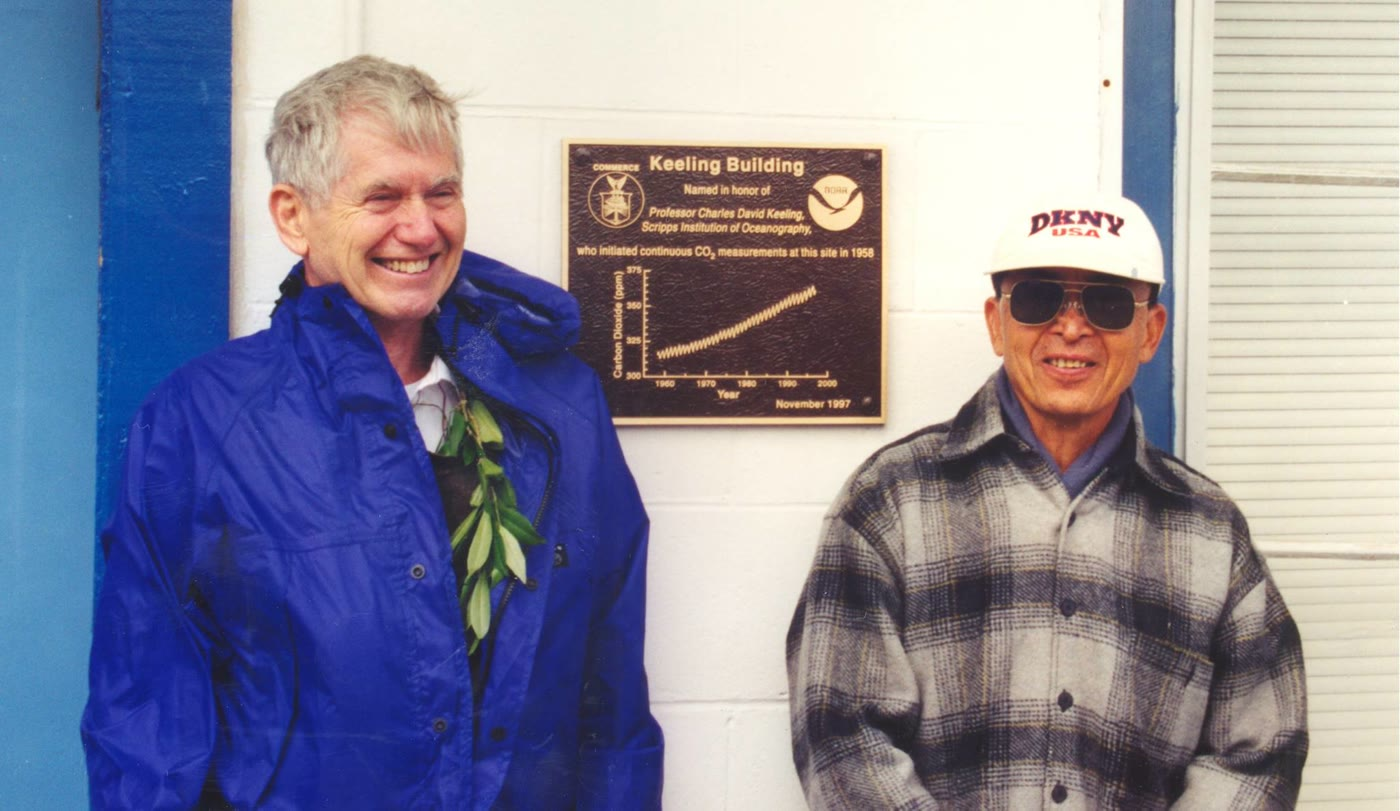
\includegraphics[width=0.62\linewidth]{images/book2/g12-noaa-keeling-chin-1997.jpg}

{\small Charles David Keeling (à gauche) et John Chin à l'observatoire du
Mauna Loa en 1997, à côté de la plaque qui donne à un bâtiment le nom de
Keeling. Photographie~: John Miller, NOAA (domaine public).}
\end{center}
\end{history}

\section{Exercices}

\begin{exercise}[$\star$]\label{exo:g12:climate-change:1}
Qu'est-ce que le \omterm{def:g12:climate-change:forcing}{forçage radiatif} d'un changement du système climatique~?
En quelle unité le mesure-t-on, et que signifie son signe~?
\end{exercise}

\begin{exercise}[$\star$]\label{exo:g12:climate-change:2}
En quel mois de l'année la concentration de dioxyde de carbone au Mauna Loa
est-elle la plus haute, et en quel mois la plus basse~? Expliquer
l'oscillation annuelle.
\end{exercise}

\begin{exercise}[$\star$]\label{exo:g12:climate-change:3}
Dans le vocabulaire des évaluations, quelle probabilité \emph{très
probable} désigne-t-il~? Et \emph{probable}~? Que signifie une fourchette
écrite $[0.95 \text{ à } 1.20]$~?
\end{exercise}

\begin{exercise}[$\star$]\label{exo:g12:climate-change:4}
Quelle part de l'énergie supplémentaire gagnée par le système climatique au
cours des dernières décennies est allée dans l'océan~? Pourquoi cela
explique-t-il que le niveau de la mer monte même sans fonte des glaces~?
\end{exercise}

\begin{exercise}[$\star$]\label{exo:g12:climate-change:5}
Donner deux \omterm{def:g12:climate-change:feedback}{rétroactions climatiques} positives et la réponse négative qui
limite le réchauffement. Expliquer chacune en une phrase.
\end{exercise}

\begin{exercise}[$\star\star$]\label{exo:g12:climate-change:6}
La concentration moyenne annuelle de dioxyde de carbone au Mauna Loa était
de \qty{315.98}{ppm} en 1959 et de \qty{427.35}{ppm} en 2025. De combien de
ppm, et de quel pourcentage, a-t-elle augmenté~? Quelle a été la hausse
moyenne par an sur toute la période~?
\end{exercise}

\begin{exercise}[$\star\star$]\label{exo:g12:climate-change:7}
Utiliser la loi logarithmique du chapitre, avec $F_{2\times} =
\qty{3.93}{W/m^2}$ et $C_0 = \qty{278}{ppm}$, pour calculer le \omterm{def:g12:climate-change:forcing}{forçage} du
dioxyde de carbone à \qty{427.35}{ppm}, la moyenne annuelle de 2025.
\end{exercise}

\begin{exercise}[$\star\star$]\label{exo:g12:climate-change:8}
Au rythme de \qty{3.7}{mm} par an, celui de 2006--2018, de combien le
niveau de la mer monterait-il en 30 ans~? Combien de fois ce rythme est-il
plus rapide que celui de 1901--1971, \qty{1.3}{mm} par an~?
\end{exercise}

\begin{exercise}[$\star\star$]\label{exo:g12:climate-change:9}
À l'aide de $\Delta T = F/\lambda$ avec $\lambda = \qty{1.16}{W.m^{-2}.\degreeCelsius^{-1}}$,
calculer le réchauffement à l'équilibre que produirait le \omterm{def:g12:climate-change:forcing}{forçage} humain
total de 2019, \qty{2.72}{W/m^2}. Le réchauffement observé d'origine
humaine n'est que d'environ \qty{1.07}{\degreeCelsius}. Donner la
principale raison de cette différence.
\end{exercise}

\begin{exercise}[$\star\star$]\label{exo:g12:climate-change:10}
Le Soleil et les volcans ont modifié la température mondiale entre
1850--1900 et 2010--2019 de $-0.1$ à $+\qty{0.1}{\degreeCelsius}$, alors
que le réchauffement observé était d'environ \qty{1.06}{\degreeCelsius}.
Que peut-on en conclure~? Quelle autre cause naturelle faut-il aussi
écarter, et que dit l'évaluation à son sujet~?
\end{exercise}

\begin{exercise}[$\star\star$]\label{exo:g12:climate-change:11}
À l'aide du tableau des \omterm{def:g12:climate-change:scenario}{projections}, dans quels \omterm{def:g12:climate-change:scenario}{scénarios} le réchauffement
de 2081--2100 restera-t-il très probablement inférieur à
\qty{2}{\degreeCelsius}~? Dans lesquels dépassera-t-il très probablement
\qty{2}{\degreeCelsius}~?
\end{exercise}

\begin{exercise}[$\star\star\star$]\label{exo:g12:climate-change:12}
Les aérosols ont produit un \omterm{def:g12:climate-change:forcing}{forçage} d'environ $-0.22$ et $\qty{-0.84}{W/m^2}$
(par la lumière solaire et par les nuages). Si l'on retirait de l'air tous
les aérosols, tout le reste restant comme en 2019, que deviendrait le
\omterm{def:g12:climate-change:forcing}{forçage} humain total~? De combien le réchauffement à l'équilibre
augmenterait-il, avec
$\lambda = \qty{1.16}{W.m^{-2}.\degreeCelsius^{-1}}$~?
\end{exercise}

\begin{exercise}[$\star\star\star$]\label{exo:g12:climate-change:13}
Montrer, à partir de la loi logarithmique, que passer de \qty{278}{ppm} à
\qty{556}{ppm} et passer de \qty{556}{ppm} à \qty{1112}{ppm} ajoutent le
même \omterm{def:g12:climate-change:forcing}{forçage}. Quel est le \omterm{def:g12:climate-change:forcing}{forçage} total à \qty{1112}{ppm}~?
\end{exercise}

\begin{exercise}[$\star\star\star$]\label{exo:g12:climate-change:14}
Dériver la loi logarithmique par rapport à $C$. Quel \omterm{def:g12:climate-change:forcing}{forçage} un ppm
supplémentaire de dioxyde de carbone ajoute-t-il à \qty{280}{ppm}, et à
\qty{420}{ppm}~? Commenter.
\end{exercise}

\begin{exercise}[$\star\star\star$]\label{exo:g12:climate-change:15}
Sans aucune \omterm{def:g12:climate-change:feedback}{rétroaction} autre que le rayonnement supplémentaire vers
l'espace, $\lambda_0 = \qty{3.22}{W.m^{-2}.\degreeCelsius^{-1}}$. Calculer
le réchauffement pour un doublement du dioxyde de carbone
($F_{2\times} = \qty{3.93}{W/m^2}$) avec $\lambda_0$, puis avec
$\lambda = \qty{1.16}{W.m^{-2}.\degreeCelsius^{-1}}$. De quel facteur les
\omterm{def:g12:climate-change:feedback}{rétroactions} amplifient-elles le réchauffement~?
\end{exercise}

\section{Problème~: la courbe de Keeling en chiffres}

\begin{problem}[{Problème du week-end --- de la respiration annuelle de la
végétation à l'année où un doublement serait atteint}]
\label{pb:g12:climate-change:1}
% ledger: data:co2-mlo (annual means 1960 316.91, 1970 325.68, 2015 401.01,
% 2025 427.35; seasonal departures May +3.37, September -3.51, means of
% 2015-2024; all from figdata/grade-12/climate_records.py), noaa:mlo-site,
% ipcc:erf-2xco2, ipcc:ecs, ipcc:feedbacks, ipcc:co2-2myr
Un élève télécharge l'enregistrement du Mauna Loa et le traite avec un
tableur. Sur 2015--2024, la concentration mensuelle se situe en moyenne
\qty{3.37}{ppm} au-dessus de la tendance lissée en mai et \qty{3.51}{ppm}
au-dessous en septembre. Les moyennes annuelles sont de \qty{316.91}{ppm}
en 1960, \qty{325.68}{ppm} en 1970, \qty{401.01}{ppm} en 2015 et
\qty{427.35}{ppm} en 2025. La concentration de 1750 était de
\qty{278}{ppm}. Utiliser la loi logarithmique avec
$F_{2\times} = \qty{3.93}{W/m^2}$.

\medskip
\noindent\textbf{Partie I --- La respiration de la végétation.}
\begin{enumerate}
  \item Quelle est l'amplitude, du maximum au minimum, du cycle annuel~?
  \item Expliquer pourquoi la concentration est la plus haute en mai et la
        plus basse en septembre.
  \item Le cycle est bien plus faible dans l'air de l'hémisphère Sud.
        Proposer une explication.
  \item Pourquoi l'observatoire a-t-il été construit à \qty{3397}{m}
        d'altitude, sur un volcan au milieu du Pacifique~?
\end{enumerate}

\medskip
\noindent\textbf{Partie II --- La tendance.}
\begin{enumerate}[resume]
  \item Calculer la hausse moyenne, en ppm par an, sur 1960--1970.
  \item La calculer sur 2015--2025.
  \item De quel facteur le rythme de hausse a-t-il augmenté~?
  \item De quel pourcentage la concentration a-t-elle augmenté entre 1750
        et 2025~?
  \item Les \omterm{def:g12:past-climates:ice-core}{carottes de glace} ne montrent jamais plus d'environ
        \qty{300}{ppm} au cours des 800\,000 dernières années. De combien
        de ppm la valeur de 2025 dépasse-t-elle ce niveau~?
\end{enumerate}

\medskip
\noindent\textbf{Partie III --- Le forçage.}
\begin{enumerate}[resume]
  \item Calculer le \omterm{def:g12:climate-change:forcing}{forçage} du dioxyde de carbone en 2025.
  \item Le calculer en 1960, ainsi que l'augmentation du \omterm{def:g12:climate-change:forcing}{forçage} entre 1960
        et 2025.
  \item Quelle concentration ajouterait \qty{1}{W/m^2} au \omterm{def:g12:climate-change:forcing}{forçage} de
        2025~?
  \item Au rythme de hausse de 2015--2025, combien d'années cela
        prendrait-il~?
\end{enumerate}

\medskip
\noindent\textbf{Partie IV --- Le doublement.}
\begin{enumerate}[resume]
  \item Quelle est la concentration correspondant à un doublement de la
        valeur de 1750~? Quel \omterm{def:g12:climate-change:forcing}{forçage} produit-elle~?
  \item Avec la meilleure estimation de la \omterm{def:g12:climate-change:ecs}{sensibilité climatique à
        l'équilibre}, quel réchauffement à l'équilibre provoquerait-elle~?
        Donner la fourchette probable.
  \item Quel paramètre de \omterm{def:g12:climate-change:feedback}{rétroaction} $\lambda$ une sensibilité de
        \qty{3}{\degreeCelsius} implique-t-elle~? Le comparer à la valeur
        \qty{1.16}{W.m^{-2}.\degreeCelsius^{-1}} obtenue en additionnant
        les \omterm{def:g12:climate-change:feedback}{rétroactions}.
  \item Pourquoi la surface n'atteindrait-elle pas ce réchauffement le jour
        même où le doublement serait atteint~?
  \item Pourquoi un calcul qui prolonge simplement le rythme de hausse
        actuel est-il un \omterm{def:g12:climate-change:scenario}{scénario}, et non une \omterm{def:g12:climate-change:scenario}{projection} du type de celles
        que font les évaluations~?
  \item Si le rythme de hausse de 2015--2025 restait le même, en quelle
        année le doublement de la concentration de 1750 serait-il atteint~?
\end{enumerate}
\end{problem}
